\documentclass[12pt, a4paper]{article}
% \setlength{\parindent}{0pt} 
% \setlength{\parskip}{1em}
\usepackage[utf8]{inputenc}
\usepackage[polish]{babel}
\addto\captionspolish{
  \renewcommand{\figurename}{Diagram}
}
\usepackage[T1]{fontenc}
\usepackage[colorlinks=true, linkcolor=black, urlcolor=blue]{hyperref}
\usepackage{pdfpages}
\usepackage[titletoc,title]{appendix}
\usepackage[nohyperlinks]{acronym}

\title{Master's Thesis on Big Data}
\author{Paweł Safuryn}
\date{2023}


\begin{document}


\includepdf[pages=-]{praca_koncowa_strona_tytulowa_BD.pdf}

\tableofcontents
\newpage

\section*{Akronimy}
\addcontentsline{toc}{section}{Akronimy}
\begin{acronym}
\acro{API}{Application Programming Interface}
\acro{ATP}{Association of Tennis Professionals}
\acro{AWS}{Amazon Web Services}
\acro{CLI}{Command-line Interface}
\acro{MiB}{Mebibajt (1 048 576 bajtów)}
\acro{ML}{Machine Learning}
\acro{WTA}{Women's Tennis Association}
\end{acronym}



\section{Wstęp}
Analiza danych tenisowych stanowi dynamiczne pole, w którym ewolucja sportu i rosnąca ilość dostępnych danych stwarzają nowe możliwości dla zawodników i organizacji tenisowych. W obliczu coraz większego znaczenia analizy danych w sporcie, nawet profesjonalni gracze zaczynają dostrzegać jej wartość. Jednakże, dostęp do zaawansowanej analizy danych pozostaje zarezerwowany głównie dla najbardziej zamożnych graczy, co stawia nowych zawodników w niekorzystnej sytuacji.

Celem niniejszego projektu jest zgłębienie potencjału analizy danych tenisowych oraz zbadanie sposobów, w jakie te dane mogą wpływać na rozwój zawodników, ich przygotowanie do meczów i treningów oraz na efektywność inwestycji w talenty tenisowe. Projekt skupi się również na analizie ogólnodostępnych danych tenisowych, w tym metodach pozyskiwania danych, takich jak scraping oraz oficjalne API od ITF, a także roli, jaką odgrywają społecznościowe źródła danych.

Warto zauważyć, że tenis to gra, gdzie nawet najmniejsze różnice w punktach decydują o wyniku. Dane analityczne mogą zatem stanowić kluczową różnicę między zwycięstwem a porażką.

Analiza danych pozwala również zauważyć powtarzalne wzorce, których niełatwo dostrzec podczas oglądania meczu na żywo. Przykładowo, kiedy gracze zdobywają punkty decydujące czy też w jakich momentach dokonują zwycięskich uderzeń.

W ostatnich latach (2023/2024), istotną zmianą było udostępnienie danych z systemu Hawk-Eye zawodnikom. Od dawna Hawk-Eye był używany w tenisie, jednakże teraz ATP nawiązało partnerstwo z Infosys, aby lepiej wykorzystać te dane.

Analiza danych tenisowych ma potencjał nie tylko wspierać indywidualnych zawodników, ale także pomagać narodowym organizacjom tenisowym w identyfikowaniu talentów i efektywnym rozdysponowywaniu środków na rozwój. To fascynujące pole, które może zmienić sposób, w jaki tenis jest rozumiany i rozwijany. 

% Wprowadzenie do problematyki pracy. Wstęp na zakończenie powinien zawierać cel pracy oraz zakres pracy. 
% Nie ma wymogu co do wyboru zestawu danych, niemniej, przyczyny wyboru powinny zostać opisane. Niezależnie od wielkości wybranego zbioru danych, analiza powinna być wykonana za pomocą narzędzi do przetwarzania Big Data.
% Proces Data Engineering/Science można podzielić w ogólności na kroki:
% 1. Zbieranie surowych danych
% 2. Przetwarzanie danych
% 3. Eksploracja danych
% 4. Czyszczenie danych
% 5. Modelowanie (opcjonalne)
% 6. Produkt oparty na danych (czyste dane, analiza, wyniki itp.)
% 7. Komunikacja wyników

% Zalinkuj Githuba z calym kodem włącznie z kodem ktory wygenerowal ten dokument.

% Cos a tym jak  tenis   sie teraz zmienia i jest wiecej analytiki, profesjonalni graczce decduja sie miec data analysts w swoim zespole ale moga sobie na to pozwolic tylka  najbogatsi gracze - niedostepne dla nowych zawodnikow
% Jak analytika moze pomagac i komu - zawodnicy, przygotowania do meczu, do treningow (nad czm najlepiej pracowac), ocena silnych i slabch punktow swoich i przeciwnikow. Ale takze dane pomagaja narodowym organizacja tenisowym lepiej wylapywac talenty i alokowac pieniadze w rozwoj - w ktorego zawodnika inwestowac i jak (co trenowac). Innego rodzaju dane (social media, player popularity) sa uzywane zeby zwiekszac fan engagement (out of scoper)

% Opisz jakie dane  są ogólnie dostepne na rynku (to moze byy troche literature review):
% Np. samozwancze data scraping, pierwsze proby oficialnego API scheme od ITF, duzo crowdsourcowanych danych gdzie ludzie sami ogladaja mecze i zapisuja statystyki

% - tennis is a game of very small margins - show some data how many points won difference - even if small data analytics can make a big difference between win or lose

% - Tennis is a game of repeatable patterns - can’t see watching live but can see the patterns when you look at data - e.g. when do people hit winners, at what score?

% - Where data is? ATP has hawk eyes report that players get / can buy. Some companies buy hawk eye data and correlate it with video and then sell to players

% - In tennis, the more money invested in player, the more chance they have at making it - just for kick start?

%  Mention the recent changes (2023/2024) with Hawk-Eye data becoming available to the players. Hawk Eye has been used since .... Now ATP partnered with Infosys to make better use of that data.

% Goal to also have everything version controlled so it can be easily  reporduced (by me on another AWS instance) or by someone else. Hence, I avoided the use of GUIs and used AWS CLI and Bash scripts instead. Any Notebooks to be run on AWS Glue or EMR Notebook are also version controlled.

% https://www.atptour.com/en/news/atp-tdi-unveil-tennis-iq-analytics-platform





\section{Przegląd literatury}

\section{Opis danych}

% Opisz dane od Jeffa - ATP i WTA
% Dokladny opis tego co tam jest i jak jest skonstruowane
% Czy unikalne ID gracza nachodza sie miedzy ATP i WTA? - tak - sa te same ID miedzy ATP i WTA
% Statystyki z Futuresow nie  maja bardziej szczegolowych statystyk tak jak mecze  ATP
% Wyjasnij roznice miedzy danymi - ATP matches, Futures, Challengers
% Opisz jak duze sa te  dane - okolo 400 MiB, nie jest  to klasyczne Big Data ze wzgledu na ograniczenie AWS Academy Learner Lab. Te dane zawsze moga rosnac i byc rozszerzone np. tagged video analysis do KAŻDEGO meczu ktory ma obraz wideo dostepny.

\section{Metodologia}

\subsection{Ustawienie środowiska}
\subsubsection{AWS Academy Learner Lab i AWS CLI}
Projekt wykonywany jest z użyciem AWS Academy Learner Lab [61569] i AWS CLI version 2. AWS CLI jest konfigurowane poprzez skopiowanie ustawień AWS Academy Learner Lab (dostępnych pod przyciskiem ,,AWS Details'') do  pliku:
\begin{verbatim}
~/.aws/credentials
\end{verbatim}
AWS Academy Learner Lab generuje tymczasowe dane uwierzytelniające do AWS CLI za każdym razem, gdy jest uruchomiony co powoduje, że plik \verb|~/.aws/credentials| musi być aktualizowany.

% Add info about ~/.aws/config - default region

% TODO: check LabRole ARN for CLI - https://us-east-1.console.aws.amazon.com/iam/home?region=us-east-1#/roles/details/LabRole?section=permissions

Opis architektury Big Data i indywidualnych technologii AWS wykorzystanych podczas projektu znajduje się w sekcji \ref{sec:aws_architecture}.

\subsubsection{Narzędzia używane lokalnie}
Poniżej znajduje się lista głównych narzędzi używanych lokalnie podczas projektu:
\begin{itemize}
    \item Python (wersja 3.9) --- główny język programowania używany do przetwarzania i analizy danych.
    \item Bash --- używany do automatyzacji zadań, głównie tych wykorzystujących AWS CLI.
    \item MacTeX i \LaTeX --- używane do napisania tej pracy końcowej.
    \item GitHub i Git --- kontrola wersji. Cały kod dostępny na repozytorium \href{https://github.com/safurynp/pw-big-data-final-project}{pw-big-data-final-project}.
    \item Miniconda --- zarządzanie środowiskiem wirtualnym oraz bibliotekami programi stycznymi (np. do Pythona). Środowisko może być załadowane używając:
\begin{verbatim}
conda env create -f environment.yml
conda activate big-data-env
\end{verbatim}

\end{itemize}

\subsection{Architektura Big Data w AWS} \label{sec:aws_architecture}
Diagram \ref{fig:aws_architecture} przedstawia ogólny zarys architektury Big Data w AWS użytej w projekcie.
\begin{figure}[h]
    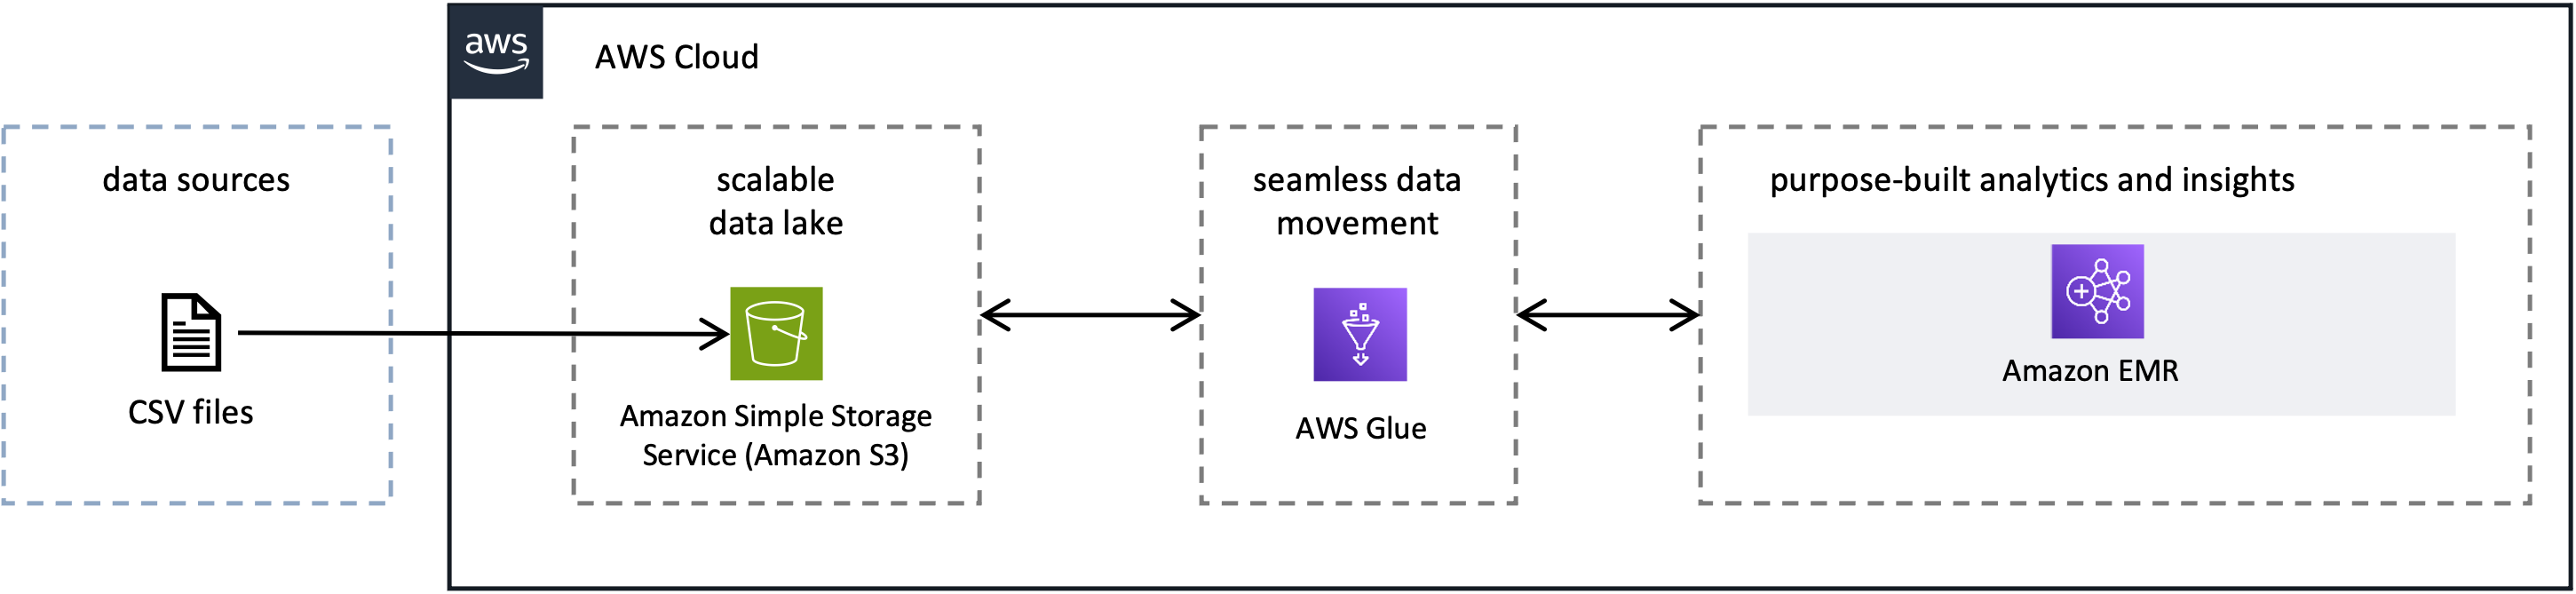
\includegraphics[width=\textwidth]{figures/aws_architecture.png}
    \caption{Architektura Big Data w AWS.}
    \label{fig:aws_architecture}
\end{figure}

Architektura ta składa się z następujących elementów:
\begin{enumerate}
    \item \textbf{Źródła danych}: Surowe dane w formacie plików CSV.
    \item \textbf{Skalowalny magazyn danych typu data lake}: 
    \begin{itemize}
        \item Amazon Single Storage Service (Amazon S3) używany do przechowywania surowych danych (bucket ,,tennis-stats-data'') oraz przetworzonych danych (bucket ,,processed-tennis-stats-data'').
        \item Crawler używany do automatycznego aktualizowania metadanych w katalogu danych.
        \item AWS Glue Data Catalog --- katalog danych używany do przechowywania metadanych o danych w Amazon S3.
    \end{itemize}
    \item \textbf{Zarządzanie przepływem danycb}: AWS Glue używany do eksploracji i przetwarzania danych za pomocą Notebooków AWS Glue i PySparka (Python API do Apache Spark).
    \item \textbf{Analityka i wizualizacja danych}: \begin{itemize}
        \item AWS QuickSight używany do wizualizacji danych i tworzenia dashboardów.
        \item Amazon EMR Notebook używany do tworzenia modeli uczenia maszynowego z użyciem PySpark ML.
    \end{itemize}

    % CloudWatch for checking logs (e.g.. of the Crawler or the AWS Glue ETL jobs)

\end{enumerate}

% Moze:
% 1. Jakis Pipeline zeby ladowal automatycznie dane z repo Jeffa do S3 bucketow
%  - moze sprawdzac regularnie czy jest nowy commit i wtedy aktualizowac wszystkie dane
% 2. Zrob jakies konrketne trasnformacje na tych danych (oczyszczanie, itd.)
% 3. Wizualizacje i analityka

\subsection{Zbieranie danych}
\subsubsection{Pozyskanie surowych danych}
Surowe tenisowe dane pozyskane są z dwóch repozytoriów na GitHubie Jeffa Sackmanna.
\begin{itemize}
    \item Dla profesjonalnego tenisa męskiego (ATP) \cite{tennis_atp}.
    \item Dla profesjonalnego tenisa żeńskiego (WTA) \cite{tennis_wta}.
\end{itemize}
Dane zostały pozyskane przez autora najprawdopodobniej (bazując na opisie repozytoriów) poprzez ekstrakcję danych (\textit{web scraping}) z Wikidata i oficjalnych stron organizacji ATP i WTA. Dane są dostępne w formacie CSV. Dane dla ATP i WTA mają ten sam format i zawierają:
\begin{itemize}
    \item Statystyki z singlowych meczów tenisowych z głównego cyklu turniejów ATP i WTA (np. Wielkie Szlemy, ATP/WTA 1000). Dostępne są dla każdego roku od 1968 (początek ery Open) do 2023. Statystyki dla każdego roku są zawarte w osobnym pliku CSV.
    \item Statystyki z singlowych meczów tenisowych z etapów eliminacji oraz z niższych rangą turniejów ATP i WTA (np. Challengers, Futures). Te dostępne są od lat 1968/1978/1991 (w zależności od rodzaju turnieju) do 2023. Statystyki dla każdego roku są zawarte w osobnym pliku CSV.
    \item Lista graczy tenisa ziemnego, którzy grali w profesjonalnym turnieju ATP lub WTA wraz z podstawowymi informacjami na ich temat.
    \item Informacje o profesjonalnym rankingu ATP i WTA (aktualizowane co tydzień) od lat 70 do 2023. Statystyki dla każdej dekady i roku 2023 są zawarte w osobnym pliku CSV.
\end{itemize}
W sumie są to 262 pliki CSV o całkowitym rozmiarze 395,7 MiB. Repozytoria Jeffa Sackmanna na GitHubie zawierają również statystyki z meczów deblowych i amatorskich ale te zostały pominięte w tym projekcie. Bardziej szczegółowy opis surowych danych znajduje się w załączniku \ref{sec:raw_data_description}.

% Napisz ile jest w sumie meczów w bazie danych, ile graczy (i ile tygodnie w rankingu, dla kazdego tygodnia pelny ranking)

% Napisz ze moje dane nie są Big Data (typowo TB danych) ze wzgledu na ograniczenia AWS Academy Learner Lab ($100). Ale są na  tyle duże, że przetwarzanie wszytskiego na raz lokalnie mogłoby być problematyczne??? Te dane mogą rosnąć i być rozszerzone np. tagged video analysis do KAŻDEGO meczu ktory ma obraz wideo dostepny.


\subsubsection{Przesyłanie danych do chmury AWS}

% TODO: Włóż różne rodzaje plików CSV do osobnych folderów

% Glue Notebook vs EMR Notebook:
% Use EMR Notebook When: You require a high level of customization, need specific big data processing frameworks, or prefer more control over cluster configurations.

% Use Glue Notebook When: You want a serverless and managed environment for ETL tasks, data exploration, and working with the Glue Data Catalog without worrying about infrastructure management.

% Both notebooks offer advantages depending on your specific use case. If your primary focus is big data processing and you need control over cluster configurations, EMR Notebook might be preferable. For ETL tasks, data catalog management, and a serverless approach, Glue Notebook could be more suitable.



% CSV files -> S3 bucket -> EMR Notebook
% Dodatkowo: CSV files -> AWS Lambda (commits) -> S3 bucket -> AWS Glue (co to robi?) -> AWS Athena (co to robi?) ->  EMR Notebook -> AWS QuickSight dashboard
% Ultimately, using AWS Transfer Family for uploading CSV files onto S3 provides a more robust, managed, and versatile solution compared to direct uploads, especially if you need to support multiple protocols, manage access control tightly, and monitor transfer activities closely.


\subsection{Eksploracja danych}
% Crawler detects three types of schema from the CSV data and ccreate as three tables. Table is the metadata definition that represents your data, including its schema -  matches, players, rankings

% Spark Notebook using Pandas (within AWS Glue Notebooks)

\subsection{Przetwarzanie i czyszczenie danych}
% Moje zastosowanie nie wymaga przetwarzania strumieniowego - przetwarzanie wsadowe jest  wystarczajace poniewaz przetwarzam dane  juz zebrane i historyczne  do moich celow biznesowych. Dane sa przetwarzane jako zbior niezaleznie od czasu ich wygenerowania. Nie potrzebuje szybkiej reakcji na dane w czasie rzeczywistym (do tego  by bylo przetwarzanie strumieniowe).

% 1. Porblematyczny tekst nie w UTF-8 w wta_matches_qual_itf_2016.csv i 2017! i 2015! -  usuń rekord ręcznie i wyślij nowy plik do S3
% 2. Napraw 'draw_size' w danych WTA - cast to long
% 3.
% Podziel score na wygrane i przegrane gemy?
% 'hand' i 'ioc' kolumny  zmienione z object na kategoryczne
% W hand zmien 'U' na NaN (U oznacza Unknown). A to Ambidextreous (oburęczny)
% Zmien daty na DateType
% Podziel score na wygrane i przegrane gemy?

% AWS Data Catalog: Create an AWS Glue Data Catalog Table: Create an AWS Glue Data Catalog table that references your parquet data files in S3. This table will provide a structured representation of your data for easy querying and analysis.

% Other AWS Glue Data Catalog benefits:
% The AWS Glue Data Catalog serves several purposes, even if your processed data in Parquet format already contains a defined schema:

% Schema Consistency and Centralized Metadata: The Glue Data Catalog acts as a centralized metadata repository. While Parquet files contain schema information, having metadata in the Glue Catalog ensures consistent and accessible metadata across various tools, queries, and users accessing the data. It also provides a structured and organized view of your data assets.

% Compatibility and Interoperability: The Glue Data Catalog integrates seamlessly with various AWS services and analytics tools. It provides a consistent interface for interacting with data across these services, promoting interoperability between different systems or users within an organization.

% Discoverability and Query Optimization: The Glue Data Catalog enables data discovery and query optimization. It stores statistics, partitioning information, and other metadata that can be utilized by query engines to optimize queries for faster execution. This metadata helps in planning and optimizing complex analytics tasks.

% Data Lineage and Governance: It allows tracking the lineage of data, understanding how it was transformed, and where it's used. This is crucial for governance, compliance, and audit purposes.

% While PySpark can infer schemas from Parquet files, using the Glue Data Catalog provides a more comprehensive and managed approach to handling metadata. It adds value in scenarios involving multiple users, tools, governance requirements, or when integrating with other AWS services where having a centralized and organized metadata repository is beneficial.


\subsection{Modelowanie matematyczne i analiza danych}

\subsubsection{Narzędzia i konfiguracja}
% Create an EMR Notebook for PySpark:
% 1. Set up an EMR lsuter: https://docs.aws.amazon.com/emr/latest/ManagementGuide/emr-gs.html
% 2. Create Studio
% 3. Create WOrkspac
% 4.. Important to launch it WITH selected cluster and using Jupyter (old), NOT JypterLab. I think I don't have permissions to launch serverless so it didn't work.
% 5.. change kernel to PySpark
%  6. Select "DefaultSecurityGroup"

% Followed this guide below to set up Python libraries (pandas, matplotlib) on EMR Cluster:
% https://aws.amazon.com/blogs/big-data/install-python-libraries-on-a-running-cluster-with-emr-notebooks/

\subsubsection{Analiza do pomocy zawodnikom i ich trenerom}
% Np. do pomocy zawodnikom  -  pokaz ktora nawierzchnia jest dla nich najlepsza a ktora najgorsza (pomaga ustawic treningi)

% Sprawdz quality  of serve zaleznosc z rankingiem - czy serwis mojego zawodnika musi byc lepszy?

\subsubsection{Analiza do pomocy narodowym organizacjom tenisowym}

\subsection{Produkt oparty na danych i komunikacja wyników}
% Napisz hipotetycznie ze moznaby swtowrzy prosty dashboard na podstawie tych danych (np. uzywajac AWS QuickSight) i udostepniec/sprzedawac go trenerom, ktoryz mogliby latwo przegladac te dane i przygotowywac specjalne treningi dla swojego zawodnika i/lub przygotowawyca zawodnika do meczu z konkretnynm przeciwnikiem na podstawie statystyk

\section{Wyniki}

\section{Wnioski i zakończenie}
% Tu należy umieścić wnioski końcowe wynikające z realizacji celu pracy dyplomowej oraz podsumowanie uzyskanych efektów. 

% Co bym zrobil wiecej
% - wlasny scaper danych albo bezposrednie poloczenie z API (ale nie ma API na stronach WTA/ATP/ITF)


% - Przeanalizuj statystyki deblowe (robilem tylko singlowe)
% - Automatyczne  testowanie kodu - np. unit  testing

% - Adding AWS Transfer Family (not avaialbe in AWS Academy Learner Lab) to upload CSV files to S3.
%   Ultimately, using AWS Transfer Family for uploading CSV files onto S3 provides a more robust, managed, and versatile solution compared to direct uploads, especially if you need to support multiple protocols, manage access control tightly, and monitor transfer activities closely.
%   Altough I didn't deal with huge amounts of data there are around  400  MiB  (Mebibytes) and I'm uploding multiple CSV files. This takes over 20 minutes to upload. This is prone to errors and an AWS Transfer Family could provide a more robust solution.
% - I could alsouse AWS Lambda to react to new commits in the repo and then start the pipeline from the beginning. Uzyc AWS Lambda zeby reagowac na nowy commit w repo - gdy przybywa nowy plik CSV to rozpoczynam caly pipeline od nowa

% - Zrobic webowa aplikacje gdzie mozna filtrowac rozne tenisowe dane - nowy git commit moglby triggerowac caly pipeline konczacy sie deployowaniem tej aplikacji z nowymi danymi. Trenerzy, institycje tenisowy moglyby latwo przegladac te dane.

% What more/better would I do:
% - video data, ball and player tracking - give examples of existing software like YOLOv3
% - You can mention the SwingVision data from my match and how it could be used

% I had problems doing my initial plan - Serverless EMR and QuickSight due to restrictions of the AWS Academy Learner Lab restrictions.

% More data cleaning - e.g WTA loser 1st serve in and serve points played


\nocite{*} % This line includes all references in the bibliography

\renewcommand{\refname}{Bibliografia}
\addcontentsline{toc}{section}{\refname}
\bibliographystyle{IEEEtran}
\bibliography{bibliography/references}

\begin{appendices}
\renewcommand{\appendixname}{Załącznik}  % Change the name to Polish

\section{Opis surowych danych} \label{sec:raw_data_description}

\end{appendices}

\end{document}